%%%%%%%%%%%%%%%%%%%%%%%%%%%%%%%%%%%%%%%%%
% Short Sectioned Assignment LaTeX Template Version 1.0 (5/5/12)
% This template has been downloaded from: http://www.LaTeXTemplates.com
% Original author:  Frits Wenneker (http://www.howtotex.com)
% License: CC BY-NC-SA 3.0 (http://creativecommons.org/licenses/by-nc-sa/3.0/)
%%%%%%%%%%%%%%%%%%%%%%%%%%%%%%%%%%%%%%%%%

% \documentclass[paper=a4, fontsize=11pt]{scrartcl} % A4 paper and 11pt font size
\documentclass[11pt, a4paper]{report}
\usepackage[T1]{fontenc} % Use 8-bit encoding that has 256 glyphs
\usepackage[utf8]{inputenc}
\usepackage{fourier} % Use the Adobe Utopia font for the document - comment this line to return to the LaTeX default
\usepackage{listings} % para insertar código con formato similar al editor
\usepackage[spanish, es-tabla]{babel} % Selecciona el español para palabras introducidas automáticamente, p.ej. "septiembre" en la fecha y especifica que se use la palabra Tabla en vez de Cuadro
\usepackage{url} % ,href} %para incluir URLs e hipervínculos dentro del texto (aunque hay que instalar href)
\usepackage{graphics,graphicx, float} %para incluir imágenes y colocarlas
\usepackage[gen]{eurosym} %para incluir el símbolo del euro
\usepackage{cite} %para incluir citas del archivo <nombre>.bib
\usepackage{enumerate}
\usepackage{hyperref}
\usepackage{graphicx}
\hypersetup{
	colorlinks=true,	% false: boxed links; true: colored links
	linkcolor=black,	% color of internal links
	urlcolor=cyan		% color of external links
}
\renewcommand{\familydefault}{\sfdefault}
\usepackage{fancyhdr} % Custom headers and footers
\pagestyle{fancyplain} % Makes all pages in the document conform to the custom headers and footers
\fancyhead[L]{} % Empty left header
\fancyhead[C]{} % Empty center header
\fancyhead[R]{Sergio Cervilla Ortega} % My name
\fancyfoot[L]{} % Empty left footer
\fancyfoot[C]{} % Empty center footer
\fancyfoot[R]{\thepage} % Page numbering for right footer
%\renewcommand{\headrulewidth}{0pt} % Remove header underlines
\renewcommand{\footrulewidth}{0pt} % Remove footer underlines
\setlength{\headheight}{13.6pt} % Customize the height of the header

\usepackage{titlesec, blindtext, color}
\definecolor{gray75}{gray}{0.75}
\newcommand{\hsp}{\hspace{20pt}}
\titleformat{\chapter}[hang]{\Huge\bfseries}{\thechapter\hsp\textcolor{gray75}{|}\hsp}{0pt}{\Huge\bfseries}

\begin{document}

	% Plantilla portada UGR
	\begin{titlepage}
\newlength{\centeroffset}
\setlength{\centeroffset}{-0.5\oddsidemargin}
\addtolength{\centeroffset}{0.5\evensidemargin}
\thispagestyle{empty}

\noindent\hspace*{\centeroffset}\begin{minipage}{\textwidth}

\centering

\includegraphics[width=0.9\textwidth]{imagenes/logo_ugr.jpg}\\[1.4cm]

\textsc{ \Large TRABAJO FIN DE GRADO\\[0.2cm]}
\textsc{ GRADO EN INGENIERIA INFORMATICA}\\[1cm]

{\Huge\bfseries Chief \\}
\noindent\rule[-1ex]{\textwidth}{3pt}\\[3.5ex]
{\large\bfseries Apoyo a la labor de la Policía Local }
\end{minipage}

\vspace{2.5cm}
\noindent\hspace*{\centeroffset}
\begin{minipage}{\textwidth}
\centering

\textbf{Autor}\\ {Sergio Cervilla Ortega}\\[2.5ex]
\textbf{Director}\\ {Juan Julián Merelo Guervós}\\[2cm]

\includegraphics[width=0.3\textwidth]{imagenes/etsiit_logo.png}\\[0.1cm]
\textsc{Escuela Técnica Superior de Ingenierías Informática y de Telecomunicación}\\
\textsc{---}\\
Granada, algún mes de 2018
\end{minipage}
\end{titlepage}

	
	% Plantilla prefacio UGR
	\chapter*{}
\thispagestyle{empty}

\begin{center}
{\large\bfseries Chief \\ Apoyo a la labor de la Policía Local}\\
\end{center}
\begin{center}
Sergio Cervilla Ortega\\
\end{center}

%\vspace{0.7cm}

\noindent{\textbf{Resumen}}\\

Lorem ipsum dolor sit amet, consectetur adipisicing elit, sed do eiusmod tempor incididunt ut labore et dolore magna aliqua. Ut enim ad minim veniam, quis nostrud exercitation ullamco laboris nisi ut aliquip ex ea commodo consequat. Duis aute irure dolor in reprehenderit in voluptate velit esse cillum dolore eu fugiat nulla pariatur. Excepteur sint occaecat cupidatat non proident, sunt in culpa qui officia deserunt mollit anim id est laborum.

\cleardoublepage

\thispagestyle{empty}

\noindent\rule[-1ex]{\textwidth}{2pt}\\[4.5ex]

D. \textbf{Juan Julián Merelo Guervós}, Profesor del Área de XXXX del Departamento de Arquitectura y Tecnología de Computadores de la Universidad de Granada.

\vspace{0.5cm}

\textbf{Informo:}

\vspace{0.5cm}

Que el presente trabajo, titulado \textit{\textbf{Chief, blah blah}},
ha sido realizado bajo mi supervisión por \textbf{Sergio Cervilla Ortega}, y autorizo la defensa de dicho trabajo ante el tribunal
que corresponda.

\vspace{0.5cm}

Y para que conste, expiden y firman el presente informe en Granada a X de mes de 2018.

\vspace{1cm}

\textbf{El director: }

\vspace{5cm}

\noindent \textbf{Juan Julián Merelo Guervós}

	
	% Índice de contenidos
	\newpage
	\tableofcontents

	% Índice de imágenes y tablas
	\newpage
	\listoffigures

	% Si hay suficientes se incluirá dicho índice
	% \listoftables 
	\newpage

	% Introducción 
	\chapter{Introducción}

Vivimos cada día en un mundo más conectado a Internet. Es una época en la que se está dejando de 
lado el lápiz y el papel, abriendo las puertas de par en par a la tecnología. Estos nuevos medios, bien
usados, son capaces de facilitarnos en numerosas ocasiones las tareas del día a día. Convierte acciones
tediosas en simples gestos que, con el tiempo, acabamos automatizando y realizamos sin esfuerzo.\\ 

\textbf{Chief} busca facilitar la labor a los agentes de policía a través del uso de la informática y las nuevas tecnologías. De esta manera, se conseguirá una mejora en la calidad del servicio de los agentes, ya que de por sí es un 
trabajo duro. Repleto de emociones y actividad física. Bajo este contexto, lo último que desea un
agente a la hora de finalizar su turno es reescribir todo el trabajo realizado a lo largo de un 
turno para pasarlo de una hoja de papel a otra, pero esta última, digital.\\ 

Bajo dicha motivación, decidí crear un sistema informatizado para facilitar las labores del cuerpo 
policial de Maracena. Una vez decidido el proyecto, procedí a reunirme con el Ayuntamiento de la 
localidad para escuchar las sugerencias de los  concejales y los policías. Así, conseguiría conocer de 
primera mano  sus inquietudes y qué les gustaría ver en el software a desarrollar.\\

La filosofía seguida en el desarrollo de dicho proyecto es una filosofía completamente \textit{open source}.
Por tanto, todo el software utilizado, así como las herramientas empleadas en su desarrollo son completamente
gratuitas y de código libre.\\ 

En este documento se presenta de manera ordenada, clara y concisa los pasos que se han seguido para
la elaboración de dicho proyecto, desde su concepción hasta la implementación. Ha sido realizado completamente por mi, Sergio Cervilla Ortega durante 
el año 2018 y es libre bajo la licencia GNU General Public License v3.0 \cite{gplv3}\\ 




	% Descripción del problema y hasta donde se llega
	\chapter{Descripción del problema}

El objetivo final que se busca con la creación de \textbf{Chief} es motivado debido a que el cuerpo policial utilizaba un esquema 
bastante anticuado para ejercer sus funciones y las convertía en tareas más complicadas, consiguiendo
una peor gestión del tiempo por parte del agente.\\

Por ejemplo, los registros de incidencias se apuntaban manualmente y al final del turno, todos los agentes se reunían para poner 
en común los datos recopilados en un documento, que posteriormente se guardaba en los ordenadores de la jefatura. Del mismo modo que en el ejemplo anterior, debían 
esperar a llegar a las dependencias para poder rellenar cualquier tipo de denuncia administrativa con los datos que habían
apuntado en un papel para que no se olvidaran.\\

Para ello, he diseñado una \textbf{aplicación web} que se encarga de gestionar una gran cantidad de 
modelos de denuncia, permitiendo que se rellenen de forma segura, a prueba de 
fallos y de una manera muy intuitiva para el usuario. Además de poder gestionar dichos documentos,
se ha creado un sistema de registro de incidencias completamente automatizado para que no se pierdan datos en ningún momento. Además de dicho sistema, se han creado un gran número de funcionalidades para ayudar a la labor de los agentes, que se explicarán en 
posteriores puntos. El Ayuntamiento de Maracena será pionero en este ámbito, ya que han sido los 
primeros que han elegido actualizarse mediante el uso de las nuevas tecnologías y una aplicación completamente libre. Una gran apuesta, pero que traerá grandes
beneficios a la calidad del trabajo del cuerpo policial y a la seguridad de los ciudadanos en su día a día. \\

A continuación se enumeran, de una manera general, los apartados que se persiguen a través de este trabajo:

\begin{enumerate}

    \item \textbf{Facilitar el trabajo a los policías locales de Maracena.}\\
    Debido a la inclusión de un sistema completamente informatizado para la elaboración de 
    denuncias administrativas, gestión de incidentes, partes de accidentes y un sistema de croquis. Consiguiendo,
    por tanto, una mejora en la productividad de los agentes y un aumento de la seguridad
    global de los datos almacenados.
    
    \item \textbf{Inclusión del software libre en organismos del estado.}\\
    Dejando a un lado herramientas privativas sobre las que no tenemos un pleno control. Con este tipo de aplicaciones, no tenemos una visión global
    de los datos que están recopilando o analizando. Además, de este modo se consigue fomentar el desarrollo libre. Porque 
    de esta manera cualquier persona puede sumarse al desarrollo y mejora de \textbf{Chief}.

    \item \textbf{Elaboración de un entorno de pruebas real.}\\
    Se persigue la creación de un entorno virtual lo más parecido posible a la 
    realidad para que el uso de la aplicación pueda ser probado antes del despliegue 
    final. Consiguiendo directamente una versión del código más robusta ante la aparición de posibles errores que se solucionarán en dicho contexto.
   	
    \item \textbf{Probar los conocimientos adquiridos a lo largo del grado.}\\
    Creando un sistema completo en el que tendremos que tener en cuenta todos los 
    aspectos técnicos adquiridos en el transcurso de la carrera. Dada la embergadura del
    proyecto, es necesario disponer de una base muy consolidada de los conocimientos adquiridos
    previamente.

    \item \textbf{Aprendizaje de tecnologías punteras en el sector.}\\
    Durante el desarollo del proyecto se ha buscado aprender y utilizar tecnologías en 
    auge que tienen un alto potencial. Esta decisión se toma en base  a la cantidad de gente
    y empresas que las utilizan, la comunidad tan amplia que tienen así como las contínuas
    mejoras que están recibiendo.  

\end{enumerate}

\section{Alcance del proyecto}

El alcance de este proyecto está centrado en llegar a una versión completamente funcional,
pero sin alcanzar la fase de producción debido a las siguientes cuestiones:

\begin{enumerate}
    \item \textbf{Cursos de formación}. Para que la aplicación sea realmente útil será necesario
    que se impartan cursos de formación tanto para los usuarios que utilizarán el sistema
    como para los administradores o gestores de la plataforma y el servidor.

    \item \textbf{Recursos materiales}. En este apartado podemos encontrar problemas como pueden
    ser la compra y configuración de servidores web, mantenimiento de los equipos informáticos, 
    compra de los dispositivos móviles en los que se ejecutará el cliente.
    
    \item \textbf{Recursos humanos}. Como puede ser la contratación del personal encargado
    de la administración de los servidores, administración y gestión de los datos de usuario , un delegado de protección de datos debido a la nueva ley \textbf{GDPR} o equipo de soporte.

\end{enumerate}



	% Estado del arte
	% 	1. Crítica al estado del arte
	% 	2. Propuesta
	\chapter{Estado del arte}

Actualmente, el estado del mercado para este tipo de desarrollos está muy limitado dado que 
la mayoría de los datos que se tratan son de carácter sensible. Por tanto, se 
debe tener un especial cuidado con el tratamiento de los mismos tanto a la hora de transmitirlos
como en su almacenamiento. Además, al ser una aplicación que será utilizada en organismos públicos 
tiene que pasar por un largo proceso burocrático ya que las acciones que se pueden realizar con este
tipo de sistemas son muy delicadas. Cualquier fallo puede causar un gran problema a uno o varios ciudadanos.\\

Por tanto, las aplicaciones orientadas a solucionar este problema son una gran minoría. En este apartado nos vamos a centrar en los dos más conocidas dentro del sector.

\section{GESPOL GPSS PDA}
La primera de las aplicaciones que encontramos es \textbf{GESPOL GPSS PDA}\cite{gespol} creada por \textit{GESPOL}. Su especialidad es el desarrollo de 
aplicaciones dedicadas específicamente a la Administración Pública.\\

Esta aplicación realiza un gran número de actividades entre ellas:

\begin{itemize}
	\item Control de acceso a usuarios.
	\item Posicionamiento GPS del agente.
	\item Gestión de incidencias.
	\item Gestión de anomalías en la vía pública.
	\item Gestión de denuncias de tráfico.
	\item Consulta a la DGT.
	\item Impresión de multas.
\end{itemize}

Este es el aspecto que tiene la aplicación: 

\begin{figure}[H]
	\centering
	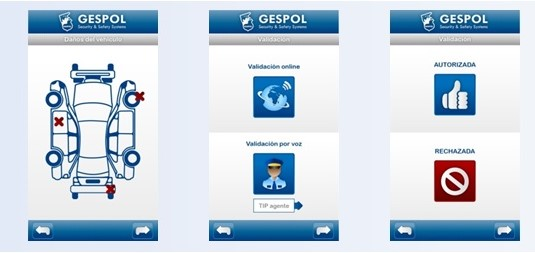
\includegraphics[scale=0.75]{imagenes/gespol2.jpg}
	\caption{Validación de usuario y daños de vehículos en GESPOL.\cite{gespol} \label{fig:figura16}}
\end{figure}

\begin{figure}[H]
	\centering
	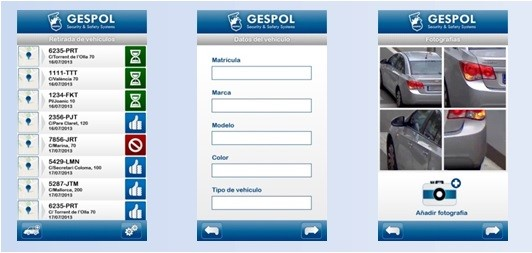
\includegraphics[scale=0.75]{imagenes/gespol1.jpg}
	\caption{Retirada, daños y fotografías de vehículos en GESPOL.\cite{gespol} \label{fig:figura17}}
\end{figure}

El principal problema de esta aplicación es que está bastante desactualizada. El desarrollo se terminó y no se han incluido mejoras en el software. Además,
es una aplicación de pago y no es de código libre, por lo que no la podemos utilizar para continuar su desarrollo con nuevas funcionalidades y adaptada a las tecnologías recientes.

\section{Appolo}
La segunda aplicación a analizar se llama \textbf{Appolo} y ha sido creada por la empresa \textit{Almerimatik Sistemas Informáticos S.A}. \\

\textit{Appolo} es un sistema informático para la gestión completa de los Cuerpos de Policía Local y afirman que es un sistema
flexible, abierto y que están en permanente evolución debido a las necesidades de sus usuarios.\\

Algunas de las funcionalidades que ofrece son las siguientes:
\begin{itemize}
	\item Gestiona el seguimiento de la actividad de los agentes.
	\item Permite completar todo el ciclo de las sanciones de ordenanza, de tráfico y de O.R.A. 
	\item Posee un módulo de sala para organizar el trabajo de los agentes.
	\item Los agentes pueden generar denuncias y partes.
	\item Es multi-entidad, por lo que se puede usar en distintas jefaturas.
\end{itemize}

En la siguiente imagen se puede comprobar los bloques en los que se compone:

\begin{figure}[H]
	\centering
	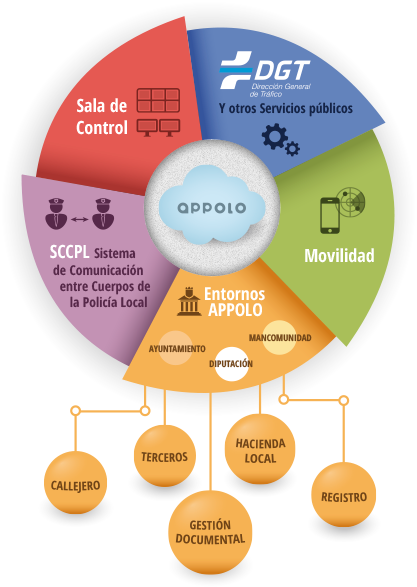
\includegraphics[scale=0.55]{imagenes/appolo-info.png}
	\caption{Bloques que conforman Appolo.\cite{appolo} \label{fig:figura15}}
\end{figure}

Esta aplicación se rige bajo una licencia \textit{open source} pero bajo pago. Por tanto, no podemos conocer el código de la aplicación
sin haber pagado por la licencia. El sistema de cobro que usan es el basado en tarifa plana, por lo cual se deberá pagar en un
único plazo y antes de comenzar a utilizar la aplicación. Esto ocasiona una gran barrera en el momento de querer comenzar a utilizar esta aplicación ya que hasta que no obtenemos la licencia, no podremos saber si se adapta a las necesidades que tenemos o si es realmente útil para los agentes.

\section{Crítica al estado del arte}

Después de analizar las aplicaciones anteriores, se puede concluir que \textbf{no} existe una aplicación
de código libre, gratuita y en la que los desarrolladores de la comunidad puedan involucrarse de manera activa.
Las aplicaciones anteriores no son muy usadas debido a su alto precio. En la mayoría de los casos, las instituciones
no pueden permitirse este gasto y no cambian el modelo que están utilizando actualmente.\\


Con esta aplicación se podrá llegar donde las anteriores aplicaciones no han llegado. De este modo al tener en cuenta un mayor sector de posibles usuarios, 
\textbf{Chief} puede conseguir una mayor implantación en el mercado. Esto puede provocar que la comunidad de desarrolladores vea una buena oportunidad y se involucre 
de manera activa en el proyecto, consiguiendo mejoras y atendiendo a las necesidades de la comunidad.

\section{Propuesta}

Se propone crear el \textbf{primer} sistema de ayuda a la labor policial de código libre y completamente gratuito que cuente
con el apoyo directo de una institución del Estado. Este proyecto puede significar una gran paso para la aceptación 
del código libre como una alternativa igual de válida que el código cerrado para un sector en el 
que hasta ahora, no ha tenido cabida.\\  


	% Análisis del problema
	% 1. Análisis de requisitos
	% 2. Análisis de las soluciones
	% 3. Solucion propuesta
	% 4. Análisis de seguridad
	\chapter{Análisis del problema}
 
 Como todo software, esta aplicación se ha diseñado y desarrollado para cubrir una
 necesidad. En base a tal necesidad, podemos crear una descripción completa de los 
 actores así como una lista de requisitos completa con la que se cubran los objetivos 
 propuestos.

\section{Descripción de los actores}
Vamos a disponer de dos actores: el \textbf{usuario} y el \textbf{administrador}. 

El \textbf{usuario} será el agente de policía que desée realizar cualquiera de las acciones
disponibles en la aplicación. Este actor no tiene por qué tener ninguna experiencia previa
con aplicaciones web pero en este escenario se les ha formado con unas nociones básicas 
a modo de tutorial de como realizar todas las acciones posibles en la aplicación y las consecuencias
que tiene en el servidor.\\

El \textbf{administrador} será la persona encargada de asegurar el correcto funcionamiento 
del software así como el encargado de la gestión de los datos de usuario y de la aplicación. Este
actor, por tanto, debe tener un alto conocimiento de las tecnologías con las que se ha construido
\textbf{Chief} para poder dar una rápida respuesta a los posibles problemas del usuario.

\section{Análisis de requisitos}

Los requisitos serán divididos en 3 tipos:

\begin{enumerate}
   \item \textbf{}
\end{enumerate}


\subsection{Requisitos funcionales}

asdadasdasdasdasds
\subsection{Requisitos no funcionales}
\subsection{Requisitos de información}


\section{Análisis de las soluciones}

\section{Solucion propuesta}

\section{Análisis de seguridad}


	% Desarrollo bajo sprints: 
	% 	1. Permitir registros y login de usuarios
	% 	3. Desarrollo del sistema de incidencias
	% 	2. Desarrollo del sistema de denuncias administrativas
	% 	3. Desarrollo del sistema de croquis

	% Resultados

	% Presupuesto

	% Conclusiones

	% Trabajos futuros


	
	\newpage
	\bibliography{bibliografia}
	\bibliographystyle{plain}
	
\end{document}

